%% DONE
\id{IRSTI 06.81.85}{https://doi.org/10.58805/kazutb.v.1.26-604}

\begin{articleheader}
\sectionwithauthors{B.N. Zhabytaу, A.K. Alpysbayeva, Sh. Niyazbekova, U.B. Ussupov, M.K. Makysh}{ANALYSIS OF INNOVATIVE ACTIVITY OF MACHINE-BUILDING INDUSTRY ENTERPRISES IN THE REPUBLIC OF KAZAKHSTAN}

{\bfseries 
\textsuperscript{1}B.N. Zhabytaу\textsuperscript{\envelope } \alink{https://orcid.org/0000-0002-9437-2619},
\textsuperscript{1}А.К. Аlpysbayeva\alink{https://orcid.org/0000-0001-6444-2148},
\textsuperscript{2}Sh. Niyazbekova\alink{https://orcid.org/0000-0002-3433-9841},
\textsuperscript{1}U.B. Ussupov\textsuperscript{\envelope } \alink{https://orcid.org/0000-0002-7706-3195},
\textsuperscript{1}M.К. Makysh\alink{https://orcid.org/0000-0001-9630-2772}}
\end{articleheader}

\begin{affiliation}
\emph{\textsuperscript{1}K.Kulazhanov Kazakh University of Technology and business, Kazakhstan, Astana,}

\emph{\textsuperscript{2}Финансовый университет при Правительстве Российской Федерации, Москва, Россия,}

\raggedright \textsuperscript{\envelope }{\em Corresponding author: \href{mailto:bayana_7778@mail.ru}{\nolinkurl{bayana\_7778@mail.ru}}, \href{mailto:nusup86@mail.ru}{\nolinkurl{nusup86@mail.ru}}}
\end{affiliation}

The innovative activity of enterprises in the field of machine-building
industry of Kazakhstan and its dynamics are considered. To give a brief
description of the current state of competitiveness of enterprises of
the machine-building industry of the Kazakhstan. Which is the main
indicator of the introduction and use of innovations. Also consider the
number of innovative enterprises in the mechanical engineering sector of
Kazakhstan and the specific weight of their innovative products.

The following research methods were used in the work: statistical,
structural functional, economic and comparative analysis.

The innovative activity of the enterprises of the machine-building
industry is an important factor for their development and
competitiveness. It allows you to introduce new technologies, improve
product quality, increase production efficiency and reduce costs.

Despite of all the advantages of innovation, many enterprises face
challenges in implementing them. One of the main problems is the lack of
financial resources for research and development. In addition,
enterprises may have difficulty finding qualified specialists who can
implement innovative projects.

Enterprises need to create a favourable environment for innovation. It
is also important to develop collaborations with other business and
scientific institutions to share experience and knowledge.

Generally, the innovative activities of enterprises of the
machine-building industry are great importance for the development of
the industry and the economy as a whole. However, for its successful
implementation, it is necessary to solve a number of problems and create
favorable conditions.

The conducted studies showed a decrease in the specific gravity of
innovative products of enterprises of the machine-building industry,
based on the peculiarities of innovative activities and the level of
innovative management of enterprises of the machine-building industry in
the region of the republic.

{\bfseries Keywords:} innovation, innovation activity, global
competitiveness index, engineering, innovation activity, innovative
products.

\begin{articleheader}
{\bfseries ҚАЗАҚСТАН РЕСПУБЛИКАСЫНДА МАШИНА ЖАСАУ ӨНЕРКӘСІБІНДЕГІ КӘСІПОРЫНДАРДЫҢ ИННОВАЦИЯЛЫҚ ҚЫЗМЕТІН ТАЛДАУ}

{\bfseries
\textsuperscript{1}Б.Н. Жабытай\textsuperscript{\envelope },
\textsuperscript{1}А.К. Алпысбаева,
\textsuperscript{2}Ш. Ниязбекова,
\textsuperscript{1}Ұ.Б. Юсупов\textsuperscript{\envelope },
\textsuperscript{1}М. Мақыш}
\end{articleheader}

\begin{affiliation}
\emph{\textsuperscript{1}Қ.Құлажанов атындағы Қазақ технология және бизнес университеті, Астана,Қазақстан,}

\emph{\textsuperscript{2}Ресей Федерациясы Үкіметі жанындағы Қаржы университеті, Мәскеу,Ресей,}

\emph{e-mail: \href{mailto:bayana_7778@mail.ru}{\nolinkurl{bayana\_7778@mail.ru}}, \href{mailto:nusup86@mail.ru}{\nolinkurl{nusup86@mail.ru}}}
\end{affiliation}

Мақаланың мақсаты Қазақстанның машина жасау өнеркәсібі саласындағы
кәсіпорындардың инновациялық белсенділігі және оның қарқыны
қарастырылады. Қазақстанның машина жасау өнеркәсібі саласы
кәсіпорындарының инновацияларды енгізу мен пайдаланудың негізгі
көрсеткіші болып табылатын бәсекеге қабілеттіліктің қазіргі жай-күйіне
қысқаша сипаттама беру. Сондай-ақ, Қазақстанның машина жасау саласындағы
инновациялық кәсіпорындардың саны және олардың инновациялық өнімдерінің
үлес салмағын қарастыру.

Жұмыста зерттеудің мына әдістері қолданылды: статистикалық, құрылымдық
функционалдық, экономикалық және салыстырмалы талдау.

Машина жасау саласы кәсіпорындарының инновациялық қызметі олардың дамуы
мен бәсекеге қабілеттілігінің маңызды факторы болып табылады. Ол жаңа
технологияларды енгізуге, өнім сапасын арттыруға және шығындарды
азайтуға мүмкіндік береді.

Инновациялардың барлық артықшылықтарына қарамасытан, көптеген
кәсіпорындар оларды енгізу кезінде проблемаларға тап болады. Басты
проблемалардың бірі зерттеулер мен әзірмелер жүргізу үшін қаржы
ресурстарының жетіспеушілігі болып табылады. Бұдан басқа, кәсіпорындарда
инновациялық жобаларды іске асыруға қабілетті білікті мамандарды іздеуде
қиындықтар туындауы мүмкін.

Кәсіпорындарға инновациялық қызмет үшін қолайлы жағдайлар жасау қажет.
Сондай-ақ тәжірибе және білім алмасу үшін басқа да іскерлік және ғылыми
мекемелермен ынтымақтастықты дамыту маңызды.

Тұтастай алған машина жасау саласы кәсіпорындарының инновациялық
қызметінің сала мен тұтастай экономиканы дамыту үшін маңызы зор. Алайда
оны табысты іске асыру үшін бірқатар проблемаларды шешу және қолайлы
жағдайлар жасау қажет.

Жүргізілген зерттеулер республиканың аймақтарында машина жасау
өнеркәсібі кәсіпорындарының инногвациялық қызметінің ерекшеліктері мен
инновациялық басқару деңгейіне сүйене отырып, машина жасау өнеркәсібі
кәсіпорындарыеың инновациялық өнімінің үлес салмағының төмендегенін
көрсетті.

{\bfseries Түйін сөздер:} инновация, инновациялық қызмет, жаһандық бәсекеге
қабілеттілік индексі, машина жасау өнеркәсібі, инновациялық белсенділік,
инновациялық өнім.

\begin{articleheader}
{\bfseries АНАЛИЗ ИННОВАЦИОННОЙ ДЕЯТЕЛЬНОСТИ ПРЕДПРИЯТИЙ МАШИНОСТРОИТЕЛЬНОЙ ПРОМЫШЛЕННОСТИ В РЕСПУБЛИКЕ КАЗАХСТАН}

{\bfseries
\textsuperscript{1}Б.Н. Жабытай\textsuperscript{\envelope },
\textsuperscript{1}А.К. Алпысбаева,
\textsuperscript{2}Ш. Ниязбекова,
\textsuperscript{1}У.Б. Юсупов\textsuperscript{\envelope },
\textsuperscript{1}М.К. Мақыш}
\end{articleheader}

\begin{affiliation}
\emph{\textsuperscript{1}Казахский университет технологии и бизнеса им. К.Кулажанова, Астана, Казахстан,}

\emph{\textsuperscript{2}Финансовый университет при Правительстве Российской Федерации, Москва, Россия,}

\emph{e-mail: \href{mailto:bayana_7778@mail.ru}{\nolinkurl{bayana\_7778@mail.ru}}, \href{mailto:nusup86@mail.ru}{\nolinkurl{nusup86@mail.ru}}}
\end{affiliation}

Целью статьи является инновационная активность предприятий в сфере
машиностроительной промышленности Казахстана и ее темпы. Дать краткую
характеристику современного состояния конкурентоспособности предприятий
отрасли машиностроительной промышленности Казахстана, являющейся
основным показателем внедрения и использования инноваций. Также
рассмотреть количество инновационных предприятий в машиностроительной
отрасли Казахстана и удельный вес их инновационной продукции.

В работе использованы следующие методы исследования: статистический,
структурно - функциональный, экономический и сравнительный анализ.

Несмотря на все приумещества инноваций, многие предприятия сталкиваются
с проблемами при их внедрении. Одной из главных проблем является
нехватка финансовых ресурсов для проведения исследования и разработок.
Кроме того, у предприятий могут возникнуть трудности с поиском
квалифицированных специалистов, способныз реализовать инновационны
проекты.

Предприятиям необходимо создать благоприятные условия для инновационной
деятельности. Также важно развивать сотрудничество с другими деловыми и
научными учреждениями для обмена опытом и занниями.

В целом инновационная деятельность предприятий машиностроительной
отрасли имеет большое занчение для развития отрасли и экономики в целом.
Однако для его успешной реализации необходимо решить ряд проблем и
создать благопрятные условия.

Проведенные исследования показали снижение удельного веса инновационной
продукции предприятий машиностроительной промышленности на основе
особенностей инногвационной деятельности и уровня инновационного
управления предприятий машиностроительной промышленности в регионах
республики.

{\bfseries Ключевые слова:} инновации, инновационная деятельность,
глобальный индекс конкурентоспособности, машиностроение, инновационная
активность, инновационная продукция.

\begin{multicols}{2}
{\bfseries Intoduction.} First of all, before proceeding to the analysis of
innovative activity of enterprises of the machine-building industry of
Kazakhstan, let's characterise he concepts of innovation and innovation
activity.

The methodological data of the National Statistical Bureau of the Agency
of Kazakhstan for Strategic Planning and Reforms (RK) provides a more
detailed detailed definition of these concepts {[}1{]}. «Innovation» is
the process of creating new ideas, technologies, products or services
that lead to improvements in existing methods, processes or products.
This may include various aspects such as scientific research,
development of new technologies, creation of new products or services,
improvement of business processes, etc. «Innovation activity» is the
process of creating, disseminating and using new ideas, technologies,
products, services and methods that lead to improvements in the
efficiency, quality and competitiveness of an organization or society as
a whole. It may include research and development, introduction of new
technologies, modernization of manufacturing processes, creation of new
products and services, adaptation of existing products and services to
changing market and consumer needs. Innovative activities can be aimed
at improving the economic, social, environmental or cultural sphere of
society.

{\bfseries Materials and methods.} V.Ghozal and other authors considered as
a productivity growth factor the significant impact of enterprise
investments on modernization and additional innovations6 especially in
the long term {[}2{]}. Maslova I.Yu. showed the importance of
qualitatively new technologies for achieving the sustainable development
of the enterprise and maintaining the covpetitiveness of its products,
as well as problems on the way to develop innovative processes and ways
to overcome them {[}3{]}. In the modern digital economy, the strategy
for the development of a modern enterprise provides for an assessment of
the need for periodic modernization and renewal of fixed assets,
technical re-equipment {[}4{]}. Tatarskikh B.Ya. and other authoars,
enterprises can take advantage of the innovative ecosystem based on
modern scientific and production platforms in all stages of the
innovation process -- from invention, material incarnation to
commercialization of a promising product {[}5{]}. Hsien Yang-Jian, Wu
Yen chun Jimm and other modeled the mechanism of innovative renewal of
fixed assets in the system of technical strategy for the development of
an engineering enterprise {[}6{]}.

The strategy of innovative activity of manufacturing enterprises is
considered by many researchers as one of the main ways to increase the
efficiency of activities that underlie an important component of the
policy of increasing competitiveness in modern conditions of rapid
implementation of the achievements of the sixth technical order. Thus,
Ambartsumyan A.E. rightly notes that industrial enterprises need to
improve their production base, external and internal logistics, adapting
them to changes in the external environment and consumer needs. Sorokin
A.V. considers the positive impact of innovations on the competitiveness
of machine-building enterprises, without losing market stability, notes
Putyatina L.M. with co-authors {[}7{]}.

For the conditions of the modern digital economy, Aminat Khagaeva and
co-authors showed the advantages of developing the production systems of
the apparatus by using the phenomenon of platformization, which provides
for a transition to more open and distributed models of innovation
{[}8{]}. According to the research of de Ruyter et al., the scale and
complexity of the architecture of digital platform innovations are
growing, the horizontal diffusion of innovative methods of production
organization to many industries is accelerating, the volume of product
innovations in production {[}9{]}.

The study used positive, normative, comparative and systematic methods
of analysis, synthesis, accumulation and scientific abstraction, as well
as a complex of mathematical and statistical methods: tabular and
graphical methods of data presentation, methods for analyzing absolute,
relative and average values, dynamic series analysis, structural
analysis, index analysis. Thanks to these research tools, the problem
under consideration is analyzed in detail in relation to specific
socio-economic conditions and processes taking place in Kazakhstan.

{\bfseries Results and discussion.} First of all, the base of any
innovation, will increase the competitiveness of the enterprise.
Therefore, briefly describing the competitiveness of domestic
enterprises, we refer to the data of the World Economic Forum (WEF),
presented in the form of annual final reports, in particular, for
2020-2022 {[}10{]}. Thus, in accordance with the annual calculations of
the Global Competitiveness Index (GIC) for 12 WEF factors for 2020-2022,
we will present the general data of the Republic of Kazakhstan (table
1).
\end{multicols}

\begin{table}[H]
\caption*{Table 1 - Тhe place of the Republic of Kazakhstan in the annual reports of housing for 2020-2022}
\centering
\begin{tabular}{|lccc|}
\hline
\multicolumn{1}{|l|}{\textbf{Indicators}}                           & \multicolumn{1}{c|}{\textbf{2020}} & \multicolumn{1}{c|}{\textbf{2021}} & \textbf{2022} \\ \hline
\multicolumn{1}{|l|}{\textbf{Global Competitiveness Index}}         & \multicolumn{1}{c|}{\textbf{59}}   & \multicolumn{1}{c|}{\textbf{59}}   & \textbf{55}   \\ \hline
\multicolumn{1}{|l|}{1. Institutes}              & \multicolumn{1}{c|}{73}  & \multicolumn{1}{c|}{61}  & 64  \\ \hline
\multicolumn{1}{|l|}{2. Infrastructure}          & \multicolumn{1}{c|}{72}  & \multicolumn{1}{c|}{69}  & 67  \\ \hline
\multicolumn{1}{|l|}{3. Information and communication technologies} & \multicolumn{1}{c|}{44}            & \multicolumn{1}{c|}{44}            & 44            \\ \hline
\multicolumn{1}{|l|}{4. Macroeconomic stability} & \multicolumn{1}{c|}{61}  & \multicolumn{1}{c|}{62}  & 60  \\ \hline
\multicolumn{1}{|l|}{5. Health}                  & \multicolumn{1}{c|}{94}  & \multicolumn{1}{c|}{97}  & 95  \\ \hline
\multicolumn{1}{|l|}{6. Education and abilities} & \multicolumn{1}{c|}{52}  & \multicolumn{1}{c|}{57}  & 57  \\ \hline
\multicolumn{1}{|l|}{7. Goods market}            & \multicolumn{1}{c|}{67}  & \multicolumn{1}{c|}{57}  & 62  \\ \hline
\multicolumn{1}{|l|}{8. Labor market}            & \multicolumn{1}{c|}{33}  & \multicolumn{1}{c|}{30}  & 25  \\ \hline
\multicolumn{1}{|l|}{9. Financial market}        & \multicolumn{1}{c|}{102} & \multicolumn{1}{c|}{100} & 104 \\ \hline
\multicolumn{1}{|l|}{10. Market size}            & \multicolumn{1}{c|}{45}  & \multicolumn{1}{c|}{45}  & 45  \\ \hline
\multicolumn{1}{|l|}{11. Business intensity}     & \multicolumn{1}{c|}{35}  & \multicolumn{1}{c|}{37}  & 35  \\ \hline
\multicolumn{1}{|l|}{12. Innovative potential}   & \multicolumn{1}{c|}{87}  & \multicolumn{1}{c|}{87}  & 95  \\ \hline
\multicolumn{4}{|l|}{\textit{Note - compiled by the author based on the literature {[}11{]}.}}               \\ \hline
\end{tabular}
\end{table}

\begin{multicols}{2}
As we see from the table, Kazakhstan's positions the GIC rating in 2022
have improved by 2 positions to 2020 over the years. The indicator of 12
factors -- «institutions» (+9), «infrastructure» (+5), «macroeconomic
stability» (+1), «good market» (+5), «labor market» (+8), positions in 5
factors in 2022 improved and compared yo 2020. Positions on 4 factors
worsened: «health» (-1), «education and abilities» (-5), «financial
market» (-2), «innovation potential» (-8). Also, the position of
Kazakhstan has not changed in terms of the factors «information and
communication technologies», «market volume» and «business intensity».

It follows from the table data that for us, depending on the subject of
the article' s research, the last two factors are the
most important -- the indicators «business intensity» and «Innovation
potential». Let' s take a closer look at the main
indicators of these factors.

The «business intensity» factor is formed from the following indicators:

1.Тhe cost of opening a business.

2.Тime to start a business.

3.Аttitude to entrepreneurial risk.

4.Readiness to delegate powers.

5.Growth of innovative companies.

6.Companies implementing destructive ideas.

7.Insolvency recovery rate.

8.Qegulatory framework on insolvency issues.

The «innovation potential» factor consists of 10 indicators:

1. Quality of research institutions.

2.Diversity of Personnel.

3. Developed clusters.

4. International joint developments.

5.Comprehensive cooperation.

6. Citation publications.

7. Order a patent.

8.Research and development costs.

9. Consumer purchasing power.

10.Order registration of a trademark.

The table below shows the place of Kazakhstan in the world ranking of
the IFI for the main indicators of these two factors (Table 2).
\end{multicols}

\begin{table}[H]
\caption*{Table 2 - The place of the Republic of Kazakhstan in the annual reports of the Global Competitiveness Index for 2020-2022}
\centering
\begin{tabular}{|lccc|}
\hline
\multicolumn{1}{|l|}{\textbf{Indicators}}                           & \multicolumn{1}{c|}{\textbf{2020}} & \multicolumn{1}{c|}{\textbf{2021}} & \textbf{2022} \\ \hline
\multicolumn{1}{|l|}{«Business intensity»}                          & \multicolumn{1}{c|}{\textbf{35}}   & \multicolumn{1}{c|}{\textbf{37}}   & \textbf{35}   \\ \hline
\multicolumn{1}{|l|}{1. The cost of starting a business}   & \multicolumn{1}{c|}{7}   & \multicolumn{1}{c|}{7}   & 7   \\ \hline
\multicolumn{1}{|l|}{2. Time to start a business}          & \multicolumn{1}{c|}{52}  & \multicolumn{1}{c|}{55}  & 23  \\ \hline
\multicolumn{1}{|l|}{3. Attitude to entrepreneurial risk}  & \multicolumn{1}{c|}{16}  & \multicolumn{1}{c|}{16}  & 14  \\ \hline
\multicolumn{1}{|l|}{4. Willingness to delegate authority} & \multicolumn{1}{c|}{71}  & \multicolumn{1}{c|}{73}  & 83  \\ \hline
\multicolumn{1}{|l|}{5. Growth of innovative companies}    & \multicolumn{1}{c|}{100} & \multicolumn{1}{c|}{103} & 107 \\ \hline
\multicolumn{1}{|l|}{6. Companies implementing destructive ideas}   & \multicolumn{1}{c|}{68}            & \multicolumn{1}{c|}{63}            & 76            \\ \hline
\multicolumn{1}{|l|}{7. The coefficient of restoration of solvency} & \multicolumn{1}{c|}{56}            & \multicolumn{1}{c|}{64}            & 64            \\ \hline
\multicolumn{1}{|l|}{8. Regulatory framework on insolvency issues}  & \multicolumn{1}{c|}{1}             & \multicolumn{1}{c|}{1}             & 1             \\ \hline
\multicolumn{1}{|l|}{«Innovative potential»}                        & \multicolumn{1}{c|}{\textbf{87}}   & \multicolumn{1}{c|}{\textbf{87}}   & \textbf{95}   \\ \hline
\multicolumn{1}{|l|}{1. Quality of research institutions}  & \multicolumn{1}{c|}{83}  & \multicolumn{1}{c|}{84}  & 82  \\ \hline
\multicolumn{1}{|l|}{2. Staff diversity}                   & \multicolumn{1}{c|}{28}  & \multicolumn{1}{c|}{50}  & 58  \\ \hline
\multicolumn{1}{|l|}{3. Developed clusters}                & \multicolumn{1}{c|}{124} & \multicolumn{1}{c|}{120} & 122 \\ \hline
\multicolumn{1}{|l|}{4. International joint developments}  & \multicolumn{1}{c|}{82}  & \multicolumn{1}{c|}{89}  & 93  \\ \hline
\multicolumn{1}{|l|}{5. Comprehensive cooperation}         & \multicolumn{1}{c|}{61}  & \multicolumn{1}{c|}{60}  & 63  \\ \hline
\multicolumn{1}{|l|}{6. Citation publications}             & \multicolumn{1}{c|}{110} & \multicolumn{1}{c|}{110} & 111 \\ \hline
\multicolumn{1}{|l|}{7. Order a patent}                    & \multicolumn{1}{c|}{79}  & \multicolumn{1}{c|}{77}  & 78  \\ \hline
\multicolumn{1}{|l|}{8. Research and development costs}    & \multicolumn{1}{c|}{95}  & \multicolumn{1}{c|}{94}  & 101 \\ \hline
\multicolumn{1}{|l|}{9. Consumer purchasing power}         & \multicolumn{1}{c|}{54}  & \multicolumn{1}{c|}{53}  & 68  \\ \hline
\multicolumn{1}{|l|}{10. Ordering trademark registration}  & \multicolumn{1}{c|}{94}  & \multicolumn{1}{c|}{94}  & 96  \\ \hline
\multicolumn{4}{|l|}{\textit{Note – compiled by the author based on the literature {[}11{]}.}}                          \\ \hline
\end{tabular}
\end{table}

\begin{multicols}{2}
As is can be seen from the table, it compared the indicators of a
decrease in the «business intensity» factor in 2022 to 2020 took place
in such indicators as «readiness for devolution» (-12), «growth of
innovative companies» (-7), «companies implementing destructive ideas»
(-8), «recovery coefficient insolvency» (-8). The indicators of the
increase are observed in the indicators «time to start a business» (+29)
and «attitude to entrepreneurial risk» (+2). And the positions on the
indicators of this factor «the cost of starting a business» and «the
regulatory framework on insolvency» have not changed.

It compared the indicators of decrease in the factor «innovation
potential» in 2022 to 2020 «diversity of personnel» (-30),
«international joint developments» (-11). «comprehensive cooperation»
(-2). «cited publications» (-1). «costs of research and development
work». It is observed in such indicators as (-6), «consumer purchasing
power level» (-14), «trademark registration order» (-2). The positions
of the increase were reflected in the indicators «quality of research
institutes» (+1), «development of clusters» (+2), «Order of patents»
(+1).

Nevertheless, it is especially important to focus on improving the
indicators of such important indicators as the growth of innovative
companies, the quality of research institutes, the development of
clusters, the publication of citations, research and development costs
among the indicators of the Global Competitiveness Index.

Thus, it can be said the given the regression of the country's
development in the GIC rating in modern economic conditions for
Kazakhstan, the presence of large reserves of mineral resources and
their high export potential is not a determining factor in the country's
competitiveness. Therefore, the father development of the economy will
depend on how quickly and timely the structural and systemic change of
the real sector of the economy occurs, where human, information and
innovative capital became the main drivers.

In addition, special attention should be paid to combating corruption in
the public and private sectors, ensuring transparency of business
processes, creating favorable conditions for doing business.

We refer to table 1 and figure 1, containing such statistical data as
data on innovative activity of enterprises of the engineering sector of
the Republic of Kazakhstan for 2019-2022, the total number of companies
with and without innovations, as well as their specific ratio (table 3,
1 picture) to study the activity of innovative activities of
enterprises.
\end{multicols}

\begin{table}[H]
\caption*{Table 3 - Innovative activity of enterprises in the field of mechanical engineering of the Republic of Kazakhstan for 2019-2022}
\centering
\begin{tabular}{|lcccc|}
\hline
\multicolumn{1}{|l|}{\textbf{Indicators}} &
  \multicolumn{1}{c|}{\textbf{2019}} &
  \multicolumn{1}{c|}{\textbf{2020}} &
  \multicolumn{1}{c|}{\textbf{2021}} &
  \textbf{2022} \\ \hline
\multicolumn{1}{|p{0.5\textwidth}|}{Total number of enterprises, units.} &
  \multicolumn{1}{c|}{337} &
  \multicolumn{1}{c|}{328} &
  \multicolumn{1}{c|}{338} &
  327 \\ \hline
\multicolumn{1}{|p{0.5\textwidth}|}{Number of enterprises with innovations, units.} &
  \multicolumn{1}{c|}{94} &
  \multicolumn{1}{c|}{73} &
  \multicolumn{1}{c|}{83} &
  77 \\ \hline
\multicolumn{1}{|p{0.5\textwidth}|}{The percentage of enterprises with innovations in the total number of enterprises} &
  \multicolumn{1}{c|}{27,89\%} &
  \multicolumn{1}{c|}{22,25\%} &
  \multicolumn{1}{c|}{24,55\%} &
  23,54\% \\ \hline
\multicolumn{1}{|p{0.5\textwidth}|}{The number of enterprises that do not have innovations, units.} &
  \multicolumn{1}{c|}{243} &
  \multicolumn{1}{c|}{255} &
  \multicolumn{1}{c|}{255} &
  250 \\ \hline
\multicolumn{1}{|p{0.5\textwidth}|}{The percentage of enterprises that do not have innovations in the total number of enterprises.} &
  \multicolumn{1}{c|}{72,11\%} &
  \multicolumn{1}{c|}{77,75\%} &
  \multicolumn{1}{c|}{75,45\%} &
  76,46\% \\ \hline
\multicolumn{5}{|l|}{Note–done by the author based on the literature {[}12{]}.} \\ \hline
\end{tabular}
\end{table}

\begin{multicols}{2}
As can be seen from the statistical data of the table, in 2021, the
share of enterprises introducing and using innovations in their
activities amounted to 23.54\% or 77 units of the total number of
enterprises consisting of 327 units. Also, these tables reflect the
negative trend of a decrease in the number of innovative enterprises in
the machine-building sector of the Republic of Kazakhstan, in
particular, over these years their physical number has decreased by 17
units and decreased in relative magnitude from 27.89\% to 23.54\%.

In the structure of the machine-building industry of Kazakhstan,
enterprises produce innovative products, working in such industries as
the production of computers, electronic and optical products; production
of electrical equipment; production of machinery and equipment not
included in other categories; production of motor vehicles, trailers and
semi-trailers; production of other vehicles.

Statistical data is relating to the share of innovative products in the
machine-building industry of the Republic of Kazakhstan in the total
number of innovative products produced in the republic for 2019-2022 are
presented from the table and figure below. It is worth to note that
against the background of a high share of the products of the industry
in question in the structure of the country' s exports,
the share of products directly improved does not exceed 5\% of the total
(Table 4, Fig. 2).
\end{multicols}

\begin{figure}[H]
	\centering
	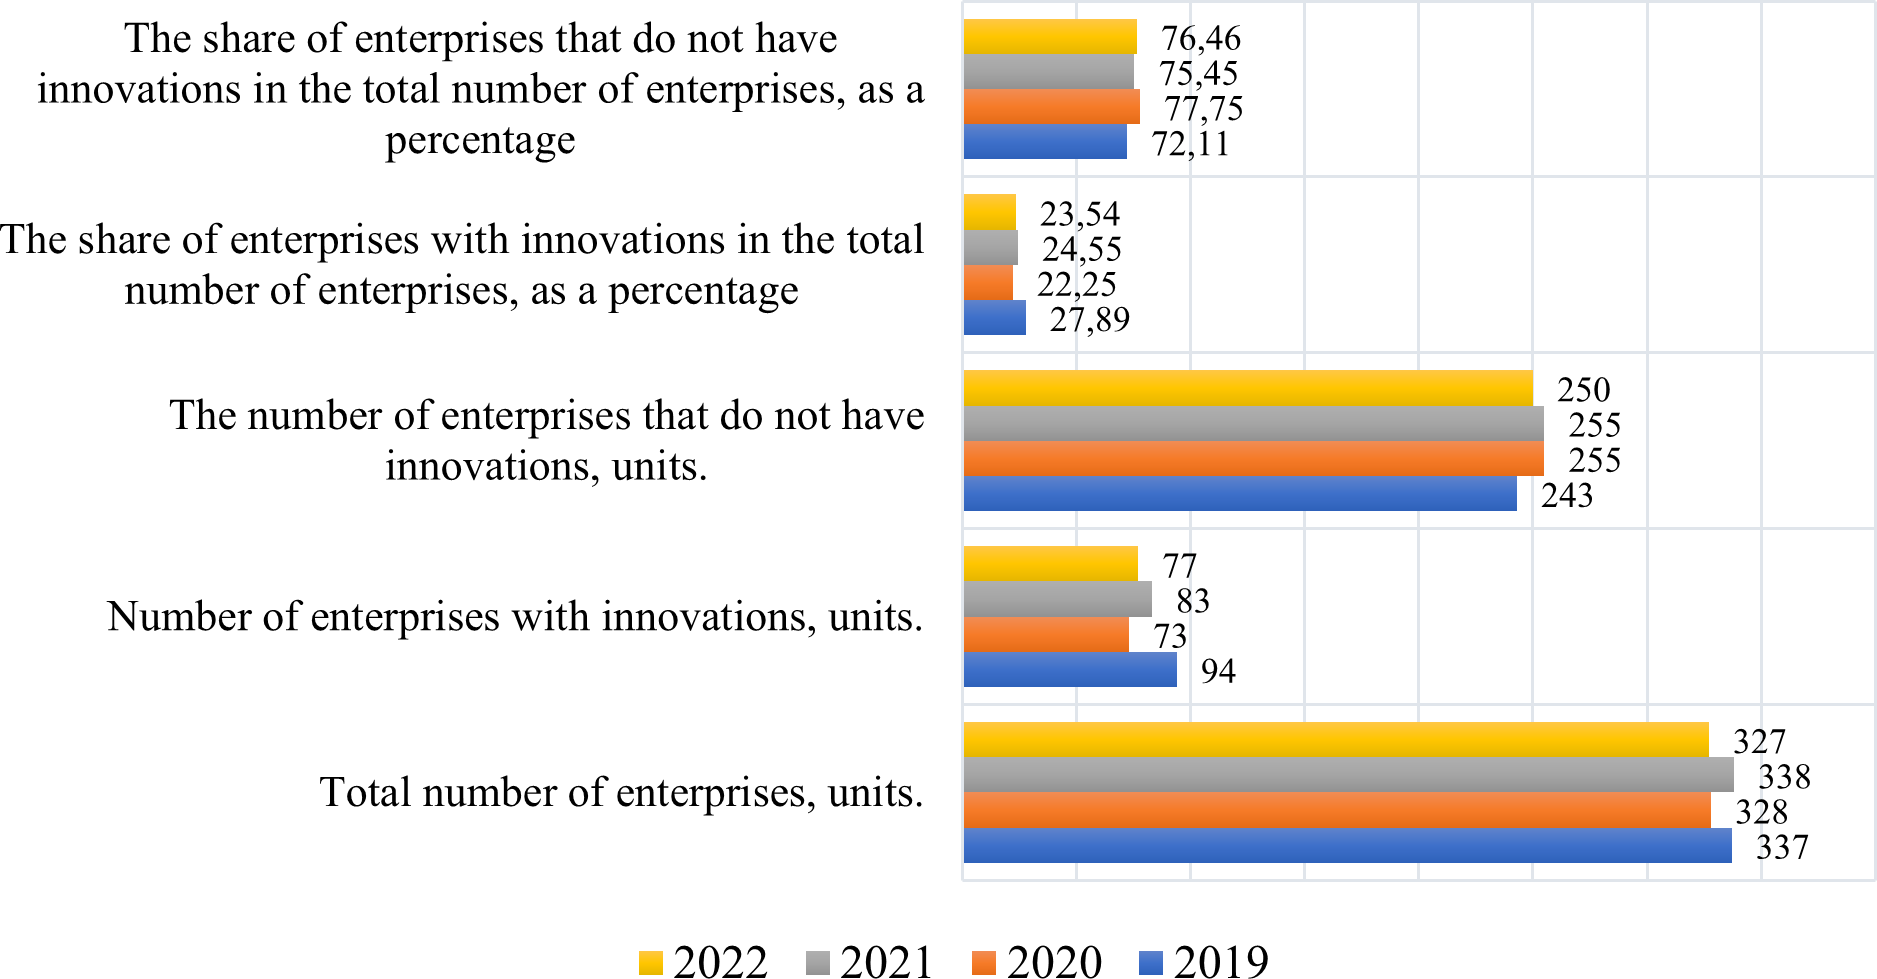
\includegraphics[width=0.8\textwidth]{media/ekon/Graph_6}
	\caption*{Figure 1 - 2019-2022 The pace of innovation activity of enterprises of the machine-building industry of the Republic of Kazakhstan}
	\caption*{\normalfont \emph{Note -- done by the author on the basis of literature {[}12{]}.}}
\end{figure}

\begin{table}[H]
\caption*{Table 4 - The share of innovative products produced by enterprises of the machine-building industry of the Republic of Kazakhstan in 2019-2022, as a percentage}
\centering
\begin{tabular}{|lcccc|}
\hline
\multicolumn{1}{|l|}{\textbf{Indicators}} &
  \multicolumn{1}{c|}{\textbf{2019}} &
  \multicolumn{1}{c|}{\textbf{2020}} &
  \multicolumn{1}{c|}{\textbf{2021}} &
  \textbf{2022} \\ \hline
\multicolumn{1}{|l|}{Machine-building industry} &
  \multicolumn{1}{c|}{29,55} &
  \multicolumn{1}{c|}{23,87} &
  \multicolumn{1}{c|}{18,55} &
  18,33 \\ \hline
\multicolumn{5}{|l|}{including:} \\ \hline
\multicolumn{1}{|l|}{Manufacture of computers, electronic and optical products} &
  \multicolumn{1}{c|}{4,36} &
  \multicolumn{1}{c|}{1,14} &
  \multicolumn{1}{c|}{0,77} &
  0,35 \\ \hline
\multicolumn{1}{|p{0.5\textwidth}|}{Manufacture of electrical} &
  \multicolumn{1}{c|}{1,58} &
  \multicolumn{1}{c|}{1,90} &
  \multicolumn{1}{c|}{1,00} &
  0,50 \\ \hline
\multicolumn{1}{|p{0.5\textwidth}|}{Equipment manufacture of machinery and equipment not included in other categories} &
  \multicolumn{1}{c|}{2,38} &
  \multicolumn{1}{c|}{1,49} &
  \multicolumn{1}{c|}{0,70} &
  0,69 \\ \hline
\multicolumn{1}{|p{0.5\textwidth}|}{Manufacture of motor vehicles, trailers and semi-trailers} &
  \multicolumn{1}{c|}{5,89} &
  \multicolumn{1}{c|}{4,98} &
  \multicolumn{1}{c|}{10,72} &
  12,73 \\ \hline
\multicolumn{1}{|p{0.5\textwidth}|}{Manufacture of other devices} &
  \multicolumn{1}{c|}{15,34} &
  \multicolumn{1}{c|}{14,36} &
  \multicolumn{1}{c|}{5,36} &
  4,06 \\ \hline
\multicolumn{5}{|l|}{\textit{Note – done by the author on the basis of literature {[}13{]}.}} \\ \hline
\end{tabular}
\end{table}


\begin{multicols}{2}
As you can see from the table, the share of innovative products produced
by enterprises in the sector of production of computers, electronic and
optical products in 2022 compared to 2015 significantly decreased from
4.36\% to 0.35\% in the structure of the machine-building industry for
the specified years. The share of innovative products produced in the
electrical equipment manufacturing sector in 2022 compared to 2019
significantly decreased from 1.58\% to 0.50\% and in the other vehicles
manufacturing sector from 15/34\% to 4.06\%, respectively. Trailers and
semi-trailers, the share of innovative products produced by enterprises
in 2022 compared to 2019 almost doubled from 5.89\% to 12.73\% in the
production of motor vehicles. At the same time, we see that in general,
in the machine-building industry, the share of the volume of innovative
products produced in the total number of innovative products producedin
the republic decreases from to year, i.e. At the same time, we see that
in general, in the machine-building industry, the share of the volume of
innovative products produced in the total number of innovative products
produced in the republic decreases from year to year, that is, in four
years the industry as a whole has lost 11.22\% of the share.
\end{multicols}

\begin{figure}[H]
	\centering
	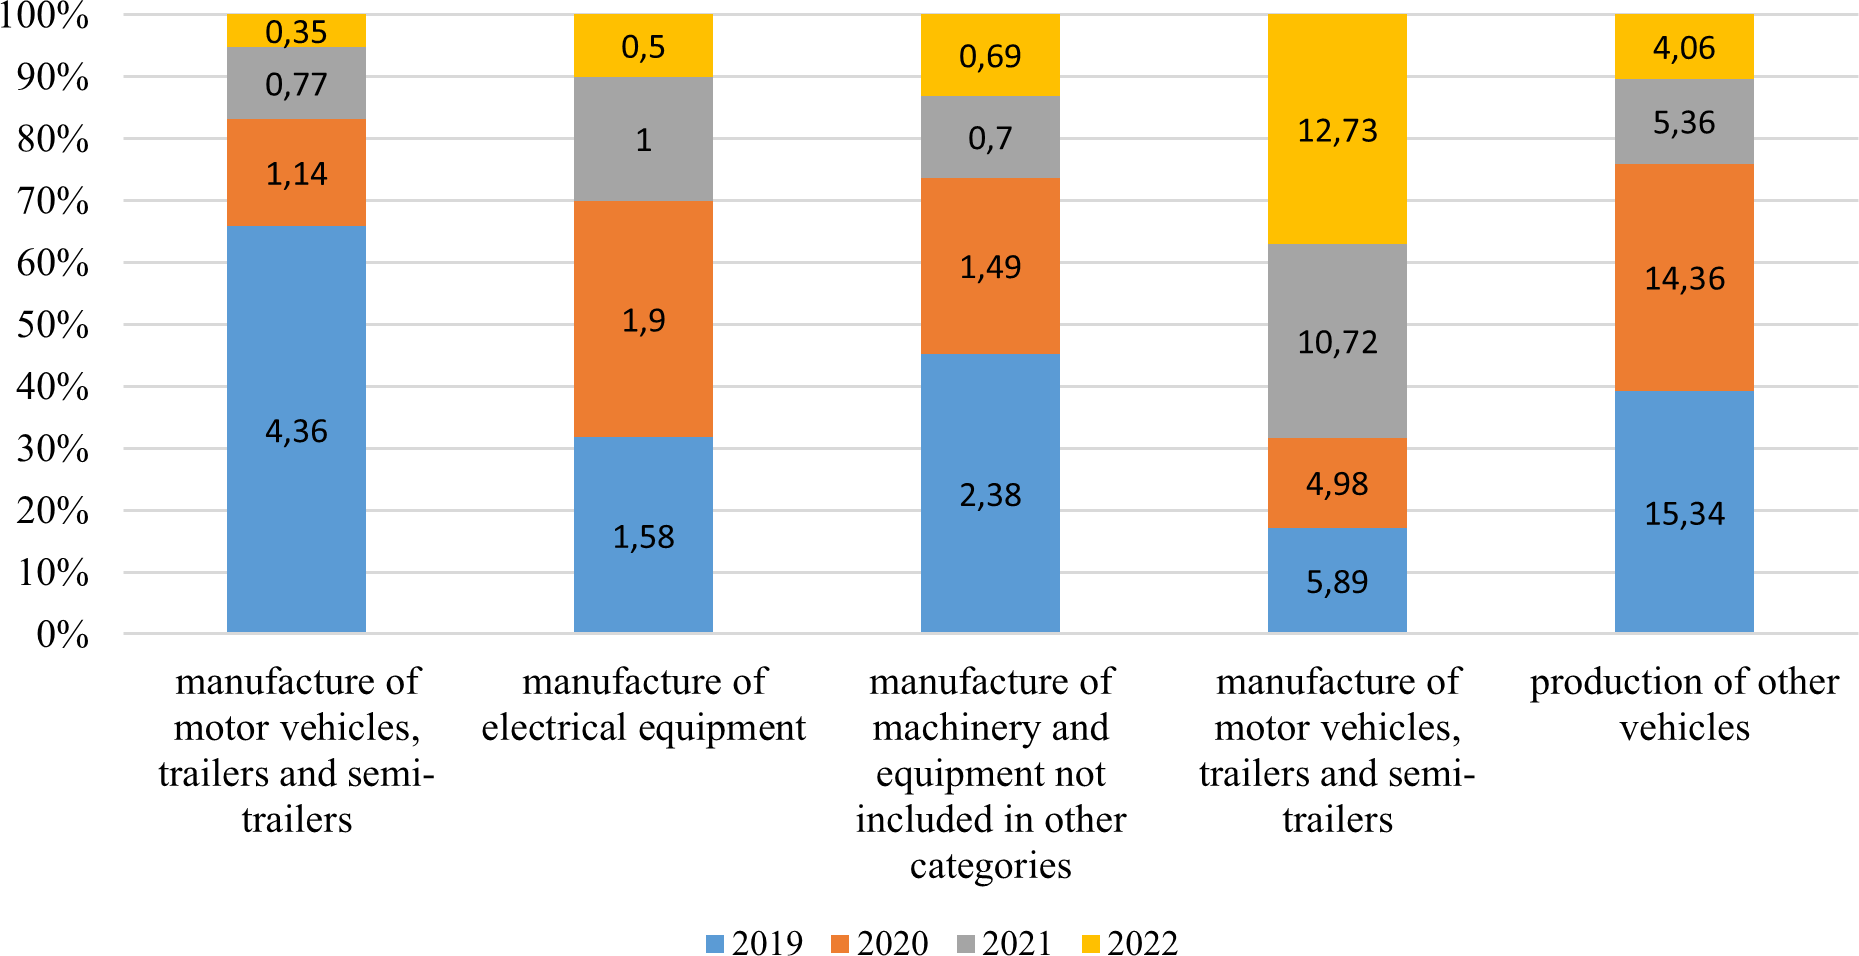
\includegraphics[width=0.8\textwidth]{media/ekon/Graph_7}
	\caption*{Figure 2 - Specific production rates of innovative products of enterprises of the machine-building industry of the Republic of Kazakhstan in 2019-2022, as a percentage}
	\caption*{\normalfont \emph{Note -- done by the author on the basis of literature{[}14{]}.}}
\end{figure}

\begin{multicols}{2}
{\bfseries Conclusions.} The innovative activity of the enterprises of the
machine-building industry is an important factor for their development
and competitiveness. It allows you to introduce new technologies,
improve product quality, increase production efficiency and reduce
costs.

Despite of all the advantages of innovation, many enterprises face
challenges in implementing them. One of the main problems is the lack of
financial resources for research and development. In addition,
enterprises may have difficulty finding qualified specialists who can
implement innovative projects {[}15{]}.

Enterprises need to create a favourable environment for innovation. It
is also important to develop collaborations with other business and
scientific institutions to share experience and knowledge.

Generally, the innovative activities of enterprises of the
machine-building industry are great importance for the development of
the industry and the economy as a whole. However, for its successful
implementation, it is necessary to solve a number of problems and create
favourable conditions.
\end{multicols}

\begin{center}
{\bfseries References}
\end{center}

\begin{references}
1. Kazakstan Respublikasy Ulttyk ekonomika ministrlіgіnіn Statistika
komitetі toragasynyn «Gylymi - zertteu zhane tazhіribelіk-konstruktorlyk
zhumystar zhane innovaciyalar statistikasy korsetkіshterіn \\kalyptastyru
bojynsha adіstemenі bekіtu turaly» 2016 zhylgy 6 kazandagy № 232 bujrygy
{[}Order of the chairman of the Statistics Committee of the Ministry of
national economy of the Republic of Kazakhstan dated October 6 on
approval of the methodology for the formation of indicators of
statistics of research and development and innovation"{]}. URL:
\href{https://www.stat.gov.kz}{https://www.stat.gov.kz} .Zhugingen kun: 13.09.2024 {[}In Kazakh{]}

2. Vivek Ghozal, Usha Nair - Reichet Investments in modernisation,
innovation and gains in productivity: Evidence from firms in the global
paper industry // Research Policy. -2009. --Vol. 38(3). -P. 536-547. DOI
10.1016/j.respol.2008.10.010.

3. L.M. Putjatina, N.V. Arsen' eva Metodicheskie aspekty
razrabotki strategii maşinostroitelnyh predpriati pri vyhode iz krizisa
// Razvitie otraslevogo i regionälnogo upravlenia. -2021. -№ 3. -S
59-65. DOI \\10.26425/1816-4277-2021-3-59-65 {[}In Russian{]}

4. Oksana E. Ivanova The Innovative Development of Industrial Production
in the Digital Economy of Russia. - 2022. DOI 10.2991/aebmr.k.220208.027

5. Streltsov A.V., Tatarskih B.Y., Yakovlev G.I. Organizational and
Economic Problems of Technical Development of the Russian Engineering //
Mediterranean Journal of Social Sciences. - 2015. -Vol 6(6).- P.509-514.
DOI 10.5901/mjss.2015.v6n6s3p509

6. Hsien Yang-Jian, Wu Yen chun Jimm Entrepreneurship through the
platform strategy in the digital era: Insights and research
opportunities // Computers in Human Behavior. - 2019. -Vol. 95. - P.
315-323. DOI 10.1016/j.chb.2018.03.033

7. Aminat Khagaeva. Innovative activity of industrial enterprises in the
context of sustainable development// 2nd International Conference on
Environmental Sustainability Management and Green Technologies \\(ESMGT
2023). -2023. -Vol. 451(5). DOI 10.1051/e3sconf/202345101022

8. Report on the Global Competitiveness Index of the World Economic
Forum (WEF GIC) for 2020. URL:
\href{https://www3.weforum.org/docs/WEF_TheGlobalCompetitivenessReport2020.pdf}{https://www3.weforum.org}.-
Date of address: 13.09.2024

9. Report on the Global Competitiveness Index of the World Economic
Forum (WEF GIC) for 2021. URL:
\href{https://www3.weforum.org/docs/WEF_Annual_Report_2020_21.pdf}{https://www3.weforum.org} .-Date
of address: 13.09.2024

10. Report on the Global Competitiveness Index of the World Economic
Forum (WEF GIC) for 2022.URL:
\href{https://www3.weforum.org/docs/WEF_Annual_Report_2021_22.pdf}{https://www3.weforum.org} .- Date
of address: 22.09.2024

11. Qazaqytannyñ ğylym jäne innovasia qyzmetı.2019-2023. Astana, 2023
statistikalyq jinağy. URL:\\
\href{https://stat.gov.kz/upload/iblock/226/1i3i3s3o3tuvvsquto0ujj0usfnji43c/\%D0\%A1-05-\%D0\%93\%20(\%D0\%BA\%D0\%B0\%D0\%B7).pdf}{https://stat.gov.kz}
- Date of address: 22.09.2024 {[}In Kazakh{]}

12. Qazaqytannyñ ğylym jäne innovasia qyzmetı.2016-2020. Nūr-Sūltan,
2020 statistikalyq jinağy.\\
\href{https://stat.gov.kz/publication/collections/?year=2020&name=16307&period=year}{https://stat.gov.kz}.-
Date of address: 22.09.2024 {[}In Kazakh{]}

13. Qazaqytannyñ ğylym jäne innovasia qyzmetı.2017-2021. Nūr-Sūltan,
2021 statistikalyq jinağy. \\Retrieved from
\href{https://stat.gov.kz/publication/collections/?year=2021&name=16307&period}{https://stat.gov.kz}.-
Date of address:22.09.2024. {[}In Kazakh{]}

14. Qazaqytannyñ ğylym jäne innovasia qyzmetı.2018-2022. Astana, 2022
statistikalyq jinağy Retrieved from
\href{https://stat.gov.kz/upload/iblock/e4a/5014j9iccdo5z0witso6spfpdbhx49ra/\%D0\%A1-10-\%D0\%93\%20(\%D0\%BA\%D0\%B0\%D0\%B7-\%D1\%80\%D1\%83\%D1\%81\%D1\%81).pdf}{https://stat.gov.kz}.-
Date of address:01.10.2024. {[}In Kazakh{]}

15. B. Zhabytay, Ş. Turmahanbetova, M. Jetesova Nūr-Sūltan qalasynyñ
infraqūrylymdyq damuynyñ \\qazırgı jağdaiyn taldau, Ekonomika i statistika
2/2020
\href{https://stat.gov.kz/upload/iblock/734/vh3mvklrnbsb6iluk2319fjas4sqcmn0/\%D0\%AD\%D0\%B8\%D0\%A1\%202\%202020.pdf}{https://stat.gov.kz}.-
Date of address: 01.10.2024. {[}In Kazakh{]}
\end{references}

\begin{authorinfo}
\emph{{\bfseries Information about the authors}}

Zhabytaу B.N. -PhD, acting Associate Professor, K.Kulazhanov Kazakh
University of Technology and Business, Astana, \\Kazakhstan, e-mail:
\href{mailto:bayana_7778@mail.ru}{\nolinkurl{bayana\_7778@mail.ru}};

Alpysbayeva A. -candidate of Economic Sciences, Аssociate professor,
K.Kulazhanov Kazakh University of Technology and Business, Astana,
Kazakhstan, e-mail:
\href{mailto:alpysbayeva.ainur77@mail.ru}{\nolinkurl{alpysbayeva.ainur77@mail.ru}}.

Niyazbekova Sh.- PhD, Associate Professor, Financial University under
the Government of the Russian Federation, Moscow, Russian
Federation,e-mail:
\href{mailto:shakizada.niyazbekova@gmail.com}{\nolinkurl{shakizada.niyazbekova@gmail.com}}.

Yussupov U.B. - PhD, Professor, K.Kulazhanov Kazakh University of
Technology and Business, Astana, Kazakhstan, e-mail:
\href{mailto:nusup86@mail.ru}{\nolinkurl{nusup86@mail.ru}};

Makysh M.К.- acting Associate Professor, K.Kulazhanov Kazakh University
of Technology and Business, Astana, Kazakhstan, e-mail:
\href{mailto:Makysh@mail.ru}{\nolinkurl{Makysh@mail.ru}};

\emph{{\bfseries Авторлар туралы мәлімет}}

Жабытай Б.Н. - PhD, и.о. асс.профессора, Казахский университет
технологии и бизнеса им.К.Кулажанова,Астана, Казахстан, e-mail:
\href{mailto:bayana_7778@mail.ru}{\nolinkurl{bayana\_7778@mail.ru}};

Алпысбаева А.К.-к.э.н. асс.профессор, Казахский университет технологии и
бизнеса им.К.Кулажанова,Астана, Казахстан, e-mail:
\href{mailto:alpysbayeva.ainur77@mail.ru}{\nolinkurl{alpysbayeva.ainur77@mail.ru}}.

Ниязбекова Ш. - PhD, доцент, Финансовый университет при Правительстве
Российской Федерации, Москва, Россия, e-mail:
shakizada.niyazbekova@gmail.com

Юсупов У. Б.- PhD, и.о.профессора, Казахский университет технологии и
бизнеса им.К.Кулажанова,Астана, Казахстан,
e-mail:\href{mailto:nusup86@mail.ru}{\nolinkurl{nusup86@mail.ru}};

Мақыш М.К. - PhD, и.о. асс.профессора, Казахский университет технологии
и бизнеса им.К.Кулажанова,Астана, Казахстан, e-mail:
Makysh\href{mailto:bayana_7778@mail.ru}{@mail.ru};
\end{authorinfo}
